\documentclass[10pt,leqno]{article}

\usepackage[%
  tmargin=1.2in,bmargin=1.2in,%
  lmargin=1.8in,rmargin=1.8in,%
]{geometry}
\usepackage{fancyhdr}
\usepackage{titlesec}
\usepackage{appendix}
\usepackage{microtype}
\usepackage[hyphens]{url}
\usepackage{enumitem}
\usepackage{xspace}
\usepackage{etoolbox}
\usepackage{ifthen}
\usepackage{tikz}
\usepackage{tikz-cd}

\usepackage{amsmath}
\definecolor{darkred}{rgb}{0.5,0.0,0.0}
\usepackage[%
  colorlinks,%
  linkcolor=darkred,%
  citecolor=darkred,%
  urlcolor=darkred,%
]{hyperref}
\usepackage{amsthm,amssymb}
% \usepackage[lining,semibold]{libertine}
% \usepackage{textcomp,stmaryrd}
% \usepackage[libertine,cmintegrals,bigdelims]{newtxmath}
% \useosf
% \usepackage[%
%   cal=boondox, calscaled=0.97,%
%   bb=boondox, bbscaled=0.98,%
% ]{mathalfa}
\usepackage{cleveref}

\frenchspacing
\urlstyle{rm}

\AtBeginDocument{%
  \setlength{\abovedisplayskip}{1.5ex plus 0.3ex minus 0.3ex}%
  \setlength{\abovedisplayshortskip}{1.0ex plus 0.3ex minus 0.3ex}%
  \setlength{\belowdisplayskip}{1.5ex plus 0.3ex minus 0.3ex}%
  \setlength{\belowdisplayshortskip}{1.0ex plus 0.3ex minus 0.3ex}%
}

\let\theoldbibliography\thebibliography
\renewcommand{\thebibliography}[1]{%
  \theoldbibliography{#1}%
  \setlength{\parskip}{0ex}
  \setlength{\itemsep}{0.5ex plus 0.2ex minus 0.2ex}
  \small
}

\pagestyle{fancy}
\renewcommand{\headrulewidth}{0pt}
\renewcommand{\footrulewidth}{0pt}
\fancyhf{}
\fancyfoot[C]{\small\thepage}

\renewcommand{\title}[1]{\newcommand{\thetitle}{#1}}
\renewcommand{\author}[1]{\newcommand{\theauthor}{#1}}
\renewcommand{\date}[1]{\newcommand{\thedate}{#1}}

\renewcommand{\maketitle}{%
  \begin{center}
    {\bfseries\MakeUppercase{%
      \thetitle}}\\[2.5ex]
    {\footnotesize\MakeUppercase{%
      \theauthor}}\\[2.5ex]
    \ifthenelse{\equal{\thedate}{}}{}{%
      \small%
      \setlength{\tabcolsep}{0.2em}%
      \begin{tabular}{rl}
        original: & \thedate \\
        updated: & \today
      \end{tabular}
    }
  \end{center}
  \vspace{2.5ex}
  \thispagestyle{fancy}
}

%%%%%%%%%%%%%%%%%%%%%%%%%%%%%%%%%%%%%%%%%%%%%%%%%%%%%%%%%%%%%%%%%%%%%%

\cspreto{section}{\setcounter{equation}{0}}

\titleformat{\section}{\centering\scshape}{\thesection.}{0.4em}{}
\titlespacing{\section}{0pt}{*4}{*1}
\titleformat{\subsection}{\scshape}{\thesubsection.}{0.4em}{}
\titlespacing{\subsection}{0pt}{*2.5}{*1}

% Display format for equations
\newcommand{\crefeqfmt}[1]{
  \crefformat{#1}{(##2##1##3)}
  \Crefformat{#1}{(##2##1##3)}
  \crefrangeformat{#1}{(##3##1##4--##5##2##6)}
  \Crefrangeformat{#1}{(##3##1##4--##5##2##6)}
  \crefmultiformat{#1}{(##2##1##3}{, ##2##1##3)}{, ##2##1##3}{, ##2##1##3)}
  \Crefmultiformat{#1}{(##2##1##3}{, ##2##1##3)}{, ##2##1##3}{, ##2##1##3)}
  \crefrangemultiformat{#1}{(##3##1##4--##5##2##6}{, ##3##1##4--##5##2##6)}{, ##3##1##4--##5##2##6}{, ##3##1##4--##5##2##6)}
  \Crefrangemultiformat{#1}{(##3##1##4--##5##2##6}{, ##3##1##4--##5##2##6)}{, ##3##1##4--##5##2##6}{, ##3##1##4--##5##2##6)}
}
% Display format for sections
\newcommand{\crefsecfmt}[1]{%
  \crefformat{#1}{\S##2##1##3}
  \Crefformat{#1}{\S##2##1##3}
  \crefrangeformat{#1}{\S\S##3##1##4--##5##2##6}
  \Crefrangeformat{#1}{\S\S##3##1##4--##5##2##6}
  \crefmultiformat{#1}{\S\S##2##1##3}{ and~##2##1##3}{, ##2##1##3}{ and~##2##1##3}
  \Crefmultiformat{#1}{\S\S##2##1##3}{ and~##2##1##3}{, ##2##1##3}{ and~##2##1##3}
  \crefrangemultiformat{#1}{\S\S##3##1##4--##5##2##6}{ and~##3##1##4--##5##2##6}{, ##3##1##4--##5##2##6}{ and~##3##1##4--##5##2##6}
  \Crefrangemultiformat{#1}{\S\S##3##1##4--##5##2##6}{ and~##3##1##4--##5##2##6}{, ##3##1##4--##5##2##6}{ and~##3##1##4--##5##2##6}
}
\crefeqfmt{equation}
\crefeqfmt{enumi}
\crefeqfmt{enumii}
\crefsecfmt{section}
\crefsecfmt{subsection}
\crefsecfmt{appendix}
\crefname{part}{Part}{Parts}
\crefname{chapter}{Chapter}{Chapters}
\crefname{figure}{Figure}{Figures}

\makeatletter

\newcommand{\thmnumfont}{\bfseries}
\newcommand{\thmheadfont}{\bfseries}
\newcommand{\thmnotefont}{\bfseries}
\newcommand{\thmhorizspace}{0.4em}

\def\swappedhead#1#2#3{%
  \thmnumber{\@upn{{\thmnumfont#2}}\@ifnotempty{#1}{.\hspace{0.25em}}}%
  \thmheadfont\thmname{#1}%
  \@ifnotempty{#3}{\ \thmnote{\thmnotefont(#3)}}%
}
\swapnumbers

\newtheoremstyle{block}%
  {2.0ex plus 0.2ex minus 0.1ex}% Space above
  {2.0ex plus 0.2ex minus 0.1ex}% Space below
  {} % Body font
  {} % Indent amount
  {\thmheadfont} % Theorem head font
  {.} % Punctuation after theorem head
  {\thmhorizspace} % Space after theorem head
  {} % Theorem head spec (can be left empty, meaning ‘normal’)

\renewenvironment{proof}[1][Proof]{\par
  \pushQED{\qed}%
  \normalfont%
  \topsep1ex plus 0.2ex minus 0.1ex\relax%
  \labelsep \thmhorizspace\relax%
  \trivlist
  \item[\hskip\labelsep\thmheadfont
    #1\@addpunct{.}]\ignorespaces
}{%
  \popQED\endtrivlist\@endpefalse%
}

\makeatother

\theoremstyle{block}

\newcommand{\defthm}[2]{%
  \newtheorem{#1}[equation]{#2}%
  \crefeqfmt{#1}%
  \newtheorem*{#1*}{#2}%
}

\defthm{algorithm}{Algorithm}
\defthm{conjecture}{Conjecture}
\defthm{construction}{Construction}
\defthm{convention}{Convention}
\defthm{corollary}{Corollary}
\defthm{definition}{Definition}
\defthm{definitions}{Definitions}
\defthm{example}{Example}
\defthm{examples}{Examples}
\defthm{exercise}{Exercise}
\defthm{fact}{Fact}
\defthm{intuition}{Intuition}
\defthm{lemma}{Lemma}
\defthm{notation}{Notation}
\defthm{nothing}{}
\defthm{proposition}{Proposition}
\defthm{question}{Question}
\defthm{remark}{Remark}
\defthm{remarks}{Remarks}
\defthm{situtation}{Situation}
\defthm{theorem}{Theorem}

\setlist{%
  leftmargin=2.5em, parsep=0ex, listparindent=\parindent,
  itemsep=1.0ex, topsep=1.0ex,%
}

\setlist[enumerate, 1]{%
  label=(\alph*),%
  ref=\alph*,%
  widest=d,%
}
\setlist[enumerate, 2]{%
  label=(\roman*),%
  ref=\theenumi.\roman*,%
}
\setlist[itemize, 1]{%
  label=$\vcenter{\hbox{\footnotesize$\bullet$}}$,%
}
\setlist[itemize, 2]{label=--}

%%%%%%%%%%%%%%%%%%%%%%%%%%%%%%%%%%%%%%%%%%%%%%%%%%%%%%%%%%%%%%%%%%%%%%

\makeatletter

\let\ea\expandafter

\newcount\foreachcount

\def\foreachletter#1#2#3{\foreachcount=#1
  \ea\loop\ea\ea\ea#3\@alph\foreachcount
  \advance\foreachcount by 1
  \ifnum\foreachcount<#2\repeat}

\def\foreachLetter#1#2#3{\foreachcount=#1
  \ea\loop\ea\ea\ea#3\@Alph\foreachcount
  \advance\foreachcount by 1
  \ifnum\foreachcount<#2\repeat}

% Roman: \rA is \mathrm{A}
\def\definerm#1{%
  \ea\gdef\csname r#1\endcsname{\ensuremath{\mathrm{#1}}\xspace}}
\foreachLetter{1}{27}{\definerm}
\foreachletter{1}{27}{\definerm}
% Script: \sA is \mathscr{A}
\def\definescr#1{%
  \ea\gdef\csname s#1\endcsname{\ensuremath{\mathscr{#1}}\xspace}}
\foreachLetter{1}{27}{\definescr}
% Calligraphic: \cA is \mathcal{A}
\def\definecal#1{%
  \ea\gdef\csname c#1\endcsname{\ensuremath{\mathcal{#1}}\xspace}}
\foreachLetter{1}{27}{\definecal}
% Bold: \bA is \mathbf{A}
\def\definebold#1{%
  \ea\gdef\csname b#1\endcsname{\ensuremath{\mathbf{#1}}\xspace}}
\foreachLetter{1}{27}{\definebold}
% Blackboard Bold: \lA is \mathbb{A}
\def\definebb#1{%
  \ea\gdef\csname l#1\endcsname{\ensuremath{\mathbb{#1}}\xspace}}
\foreachLetter{1}{27}{\definebb}
% Fraktur: \ka is \mathfrak{a}, \kA is \mathfrak{A}
\def\definefrak#1{%
  \ea\gdef\csname k#1\endcsname{\ensuremath{\mathfrak{#1}}\xspace}}
\foreachletter{1}{27}{\definefrak}
\foreachLetter{1}{27}{\definefrak}
% Sans serif: \iA \is \mathsf{A}
\def\definesf#1{%
  \ea\gdef\csname i#1\endcsname{\ensuremath{\mathsf{#1}}\xspace}}
\foreachletter{1}{6}{\definesf}
\foreachletter{7}{14}{\definesf}
\foreachletter{15}{27}{\definesf}
\foreachLetter{1}{27}{\definesf}
% Bar: \Abar is \overline{A}, \abar is \overline{a}
\def\definebar#1{%
  \ea\gdef\csname #1bar\endcsname{\ensuremath{\overline{#1}}\xspace}}
\foreachLetter{1}{27}{\definebar}
\foreachletter{1}{8}{\definebar} % \hbar is something else!
\foreachletter{9}{15}{\definebar} % \obar is something else!
\foreachletter{16}{27}{\definebar}
% Tilde: \Atil is \widetilde{A}, \atil is \widetilde{a}
\def\definetil#1{%
  \ea\gdef\csname #1til\endcsname{\ensuremath{\widetilde{#1}}\xspace}}
\foreachLetter{1}{27}{\definetil}
\foreachletter{1}{27}{\definetil}
% Hats: \Ahat is \widehat{A}, \ahat is \widehat{a}
\def\definehat#1{%
  \ea\gdef\csname #1hat\endcsname{\ensuremath{\widehat{#1}}\xspace}}
\foreachLetter{1}{27}{\definehat}
\foreachletter{1}{27}{\definehat}
% Checks: \Achk is \widecheck{A}, \achk is \widecheck{a}
\def\definechk#1{%
  \ea\gdef\csname #1chk\endcsname{\ensuremath{\widecheck{#1}}\xspace}}
\foreachLetter{1}{27}{\definechk}
\foreachletter{1}{27}{\definechk}
% Underline: \Aund is \underline{A}, \aund is \underline{a}
\def\defineul#1{%
  \ea\gdef\csname #1und\endcsname{\ensuremath{\underline{#1}}\xspace}}
\foreachLetter{1}{27}{\defineul}
\foreachletter{1}{27}{\defineul}

\makeatother

%%%%%%%%%%%%%%%%%%%%%%%%%%%%%%%%%%%%%%%%%%%%%%%%%%%%%%%%%%%%%%%%%%%%%%

\usetikzlibrary{calc,decorations.pathmorphing,shapes,arrows}
\tikzcdset{
  arrow style=tikz,
  diagrams={>={stealth}},
}

\newcommand{\arrlen}{1em}
\renewcommand{\to}{\mathrel{\tikz[baseline]%
    \draw[>=stealth,->](0,0.5ex)--(\arrlen,0.5ex);}}
\newcommand{\from}{\mathrel{\tikz[baseline]%
    \draw[>=stealth,<-](0,0.5ex)--(\arrlen,0.5ex);}}
\renewcommand{\mapsto}{\mathrel{\tikz[baseline]%
    \draw[>=stealth,|->](0,0.5ex)--(\arrlen,0.5ex);}}
\newcommand{\inj}{\mathrel{\tikz[baseline]%
    \draw[>=stealth,right hook->](0,0.5ex)--(\arrlen,0.5ex);}}
\newcommand{\surj}{\mathrel{\tikz[baseline]%
    \draw[>=stealth,->>](0,0.5ex)--(\arrlen,0.5ex);}}
\newcommand{\fromto}{\mathrel{%
  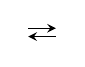
\begin{tikzpicture}[baseline]%
    \draw[>=stealth,<-](0,0.15ex)--(\arrlen,0.15ex);%
    \draw[>=stealth,->](0,0.85ex)--(\arrlen,0.85ex);%
  \end{tikzpicture}}}
\newcommand{\doubto}{\mathrel{%
  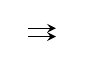
\begin{tikzpicture}[baseline]%
    \draw[>=stealth,->](0,0.15ex)--(\arrlen,0.15ex);%
    \draw[>=stealth,->](0,0.85ex)--(\arrlen,0.85ex);%
  \end{tikzpicture}}}
\newcommand{\lblto}[1]{\mathrel{%
    \begin{tikzpicture}[baseline= {( $ (current bounding box.south) + (0,-0.5ex) $ )}]
      \node[inner sep=.4ex] (a) {\,$\scriptstyle #1$\,};
      \draw[>=stealth,->] (a.south west) -- (a.south east);
    \end{tikzpicture}}}
\newcommand{\isoto}{\lblto{\sim}}

\newcommand{\simpl}[3]{
  \begin{tikzcd}[ampersand replacement=\&, column sep=small]
    #1 \&
    #2 \ar[l, shift right=0.35ex]
       \ar[l, shift left=0.35ex] \&
    #3 \ar[l, shift right=0.70ex]
       \ar[l, shift left=0.70ex]
       \ar[l] \&
    \cdots \ar[l, shift right=0.35ex]
           \ar[l, shift left=0.35ex]
           \ar[l, shift right=1.05ex]
           \ar[l, shift left=1.05ex]
  \end{tikzcd}
}
\newcommand{\cosimpl}[3]{
  \begin{tikzcd}[ampersand replacement=\&, column sep=small]
    #1 \ar[r, shift right=0.35ex]
       \ar[r, shift left=0.35ex] \&
    #2 \ar[r, shift right=0.70ex]
       \ar[r, shift left=0.70ex]
       \ar[r] \&
    #3 \ar[r, shift right=0.35ex]
       \ar[r, shift left=0.35ex]
       \ar[r, shift right=1.05ex]
       \ar[r, shift left=1.05ex] \&
    \cdots
  \end{tikzcd}
}

\newcommand{\tto}{\mathrel{\tikz[baseline]%
    \draw[>=stealth,->,double, double distance = 0.3ex](0,0.5ex)--(\arrlen,0.5ex);}}
\newcommand{\doubfrom}{\mathrel{%
  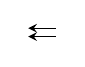
\begin{tikzpicture}[baseline]%
    \draw[>=stealth,<-](0,0.15ex)--(\arrlen,0.15ex);%
    \draw[>=stealth,<-](0,0.85ex)--(\arrlen,0.85ex);%
  \end{tikzpicture}}}
\newcommand{\tripfrom}{\mathrel{%
  
\begin{tikzpicture}[baseline]%
    \draw[>=stealth,<-](0,0.00ex)--(\arrlen,0.00ex);%
    \draw[>=stealth,<-](0,0.50ex)--(\arrlen,0.50ex);%
    \draw[>=stealth,<-](0,1.00ex)--(\arrlen,1.00ex);%
  \end{tikzpicture}}}


\renewcommand{\l}{\left}
\renewcommand{\r}{\right}
\newcommand{\f}{\frac}
\renewcommand{\o}{\overline}
\renewcommand{\u}{\underline}
\newcommand{\til}{\widetilde}
\renewcommand{\hat}{\widehat}
\newcommand{\del}{\partial}
\newcommand{\dash}{\text{-}}
\renewcommand{\c}{\colon}
\newcommand{\lc}{\,:\!}
\newcommand{\ce}{\coloneq}%{\mathrel{:=}}
\newcommand{\ec}{\eqcolon}%{\mathrel{=:}}
\newcommand{\iso}{\simeq}
\newcommand{\dual}{\vee}
\newcommand{\ldb}{\llbracket}
\newcommand{\rdb}{\rrbracket}

\newcommand{\Obj}{\operatorname{Obj}}
\newcommand{\Hom}{\operatorname{Hom}}
\newcommand{\Map}{\operatorname{Map}}
\newcommand{\Fun}{\operatorname{Fun}}
\newcommand{\Aut}{\operatorname{Aut}}
\newcommand{\Iso}{\operatorname{Iso}}
\renewcommand{\id}{\mathrm{id}}
\renewcommand{\im}{\operatorname{im}}
\newcommand{\op}{\mathrm{op}}
\newcommand{\univ}{\mathrm{univ}}
\newcommand{\colim}{\operatorname*{colim}}
\newcommand{\dlim}{\displaystyle\lim}
\newcommand{\dcolim}{\displaystyle\colim}
\newcommand{\Spec}{\operatorname{Spec}}
\newcommand{\Spf}{\operatorname{Spf}}

%%%%%%%%%%%%%%%%%%%%%%%%%%%%%%%%%%%%%%%%%%%%%%%%%%%%%%%%%%%%%%%%%%%%%%


\title{Math 216A Homework 5}
\author{Arpon Raksit}
\date{October 26, 2016}

\numberwithin{block}{section}

%%%%%%%%%%%%%%%%%%%%%%%%%%%%%%%%%%%%%%%%%%%%%%%%%%%%%%%%%%%%%%%%%%%%%%

\begin{document}
\maketitle

%%%%%%%%%%%%%%%%%%%%%%%%%%%%%%%%%%%%%%%%%%%%%%%%%%%%%%%%%%%%%%%%%%%%%%

\section{Normalization}

Let $X$ be an integral scheme.

\begin{definition}
  \label{normalization}
  We say an $X$-scheme $\pi \c \til{X} \to X$ exhibits $\til{X}$ as a \emph{normalization} of $X$ if:
  \begin{enumerate}
  \item $\til{X}$ is normal and integral, and $\pi$ is dominant;
  \item for any normal and integral scheme $Y$ and dominant map of schemes $\rho \c Y \to X$, there exists a unique map $\til{\rho} \c Y \to \til{X}$ over $X$.
  \end{enumerate}
\end{definition}

\begin{remark}
  \label{normalization-unique}
   By the usual universal property/final object/Yoneda business, a normalization of $X$ is unique up to unique isomorphism (as an $X$-scheme). So from here on out we are entitled to call something \emph{the} normalization rather than \emph{a} normalization.
\end{remark}

\begin{remark}
  \label{irreducible-dominant-generic}
  Recall (as stated on the homework for exercise 3.7) that a map $\pi \c T \to S$ of irreducible schemes is dominant if and only if it takes the generic point of $Y$ to the generic point of $S$. This in particular implies that such a $\pi$ is irreducible if and only if for any single nonempty open $U \subseteq S$ and open $V \subseteq \pi^{-1}(U)$ the restriction $\pi|_V \c V \to U$ is dominant.
\end{remark}

\begin{lemma}
  \label{normalization-restricts-to-open}
  Let $U \subseteq X$ be a nonempty open subscheme (note $U$ is still integral). Suppose given a normalization $\pi \c \til{X} \to X$ of $X$. Let $\til{U} \ce \pi^{-1}(U)$. Then the restriction $\pi|_{\til{U}} \c \til{U} \to U$ exhibits $\til{U}$ as the normalization of $U$.

  \begin{proof}
    Since $\til{U}$ is an open subscheme of $\til{X}$, it's clear that $\til{U}$ is normal and integral. And since $U$ is nonempty it is immediate from \cref{irreducible-dominant-generic} that the restriction $\pi|_{\til{U}}$ remains dominant.

    Now suppose given a dominant map of schemes $\rho \c Y \to U$ with $Y$ normal and integral. The composite $Y \to U \inj X$ factors uniquely through $\pi \c \til{X} \to X$, so it's clear that $\rho$ factors uniquely through $\pi|_{\til{U}} \c \til{U} \to Y$.
  \end{proof}
\end{lemma}

\begin{proposition}
  \label{normalization-glues-from-opens}
  Let $\{U_i\}_{i \in I}$ be an cover of $X$ by nonempty opens. Suppose given normalizations $\pi_i \c \til{U}_i \to U_i$ of $U_i$ for each $i \in I$. Then these glue to a map $\pi \c \til{X} \to X$ exhibiting $\til{X}$ as the normalization of $X$.

  \begin{proof}
    To construct $\pi \c \til{X} \to X$, we need to exhibit isomorphisms
    \[
      \phi_{i,j} \c \pi_i^{-1}(U_i \cap U_j) \isoto \pi_j^{-1}(U_i \cap U_j)
    \]
    that are coherent in the usual sense. But this data comes to us immediately from the fact that normalizations restrict well to open subschemes \cref{normalization-restricts-to-open} together with the uniqueness of normalization up to unique isomorphism \cref{normalization-unique}.

    By construction $\til{X}$ has an open cover by normal integral schemes, hence itself is a normal integral scheme. And $\pi$ is dominant by \cref{irreducible-dominant-generic}.

    Suppose given a dominant map of schemes $\rho \c Y \to X$ with $Y$ normal and integral. For $i \in I$, let $Y_i \ce \rho^{-1}(U_i)$ and let $\rho_i \ce \rho|_{Y_i} \c Y_i \to U_i$ denote the restriction. Then each $Y_i$ is an open subscheme of $Y$, hence normal and integral, and by \cref{irreducible-dominant-generic} $\rho_i$ is dominant, so we obtain unique maps $\til{\rho}_i \c Y_i \to \til{U}_i$ over $U_i$. As noted in the construction of $\til{X}$, by \cref{normalization-restricts-to-open} the intersection $\til{U}_i \cap \til{U}_j$ in $\til{X}$ is the normalization of $U_i \cap U_j$. Thus the two maps
    \[
      \til{\rho}_i|_{Y_i \cap Y_j}, \til{\rho}_j|_{Y_i \cap Y_j} \c Y_i \cap Y_j \to \til{U}_i \cap \til{U}_j,
    \]
    both lifting $\rho|_{Y_i \cap Y_j} \c Y_i \cap U_j \to U_i \cap U_j$, must be equal. Hence we may glue the lifts $\til{\rho}_i$ to obtain a lift $\til{\rho} \c Y \to \til{X}$ of $\rho$. The lift is unique since the lifts $\til{\rho}_i$ were unique. Thus $\til{X}$ is indeed the normalization of $X$.
  \end{proof}
\end{proposition}

\begin{nothing}
  \label{normalization-affine}
  Now suppose $X$ is an affine scheme $\Spec A$, still integral so $A$ is a domain. Let $K$ be the field of fractions of $A$.

  \begin{sublemma}
    \label{normal-domain}
    The following are equivalent:
    \begin{enumerate}
    \item \label{normal-domain-global} $A$ is integrally closed in $K$.
    \item \label{normal-domain-prime} $X$ is normal, i.e. for all prime ideals $\kp$ in $A$, $A_\kp$ is integrally closed in $K$.
    \item \label{normal-domain-max} For all maximal ideals $\km$ in $A$, $A_\km$ is integrally closed in $K$.
    \end{enumerate}

    \begin{proof}
      Some commutative algebra, omitted here.
    \end{proof}
  \end{sublemma}

  \begin{subproposition}
    \label{normalization-affine-prop}
    Let $\til{A}$ be the integral closure of $A$ in $K$. Let $\til{X} \ce \Spec \til{A}$. Then the map $\pi \c \til{X} \to X$ induced by the inclusion $\pi^\sharp \c A \inj \til{A}$ exhibits $\til{X}$ as the normalization of $X$.

    \begin{proof}
      Obviously $\til{X}$ is integral, and by \cref{normal-domain} it's normal. And $\pi$ is dominant since $\pi^\sharp$ is injective (alternatively this follows from \cref{irreducible-dominant-generic}).

      Suppose given a dominant map of schemes $\rho \c Y \to X$ with $Y$ normal and integral. Recall that, since $X$ is affine, this is determined uniqely by the map on global sections $\rho^\sharp \c  A \to \Gamma(Y,\sO_Y)$. Since $\til{X}$ is also affine, it suffices to show that there is a unique extension $\til{\rho}^\sharp \c \til{A} \to \Gamma(Y,\sO_Y)$. Let $L$ denote the function field of $Y$, which is canonically isomorphic to the fraction field of $\Gamma(U,\sO_Y)$ for any nonempty affine open $U \subseteq Y$ by [Hartshorne, Exercise II.3.6].

      Consider the commutative diagram
      \[
        \begin{tikzcd}
          A \ar[r, "\rho^\sharp"] \ar[d] &
          \Gamma(Y,\sO_Y) \ar[d] \\
          \til{A} \ar[d] &
          \Gamma(U, \sO_Y) \ar[d] \\
          K \ar[r, "\rho^\sharp"] &
          L,
        \end{tikzcd}
      \]
       where here $U \subseteq Y$ is any nonempty affine open, the vertical maps are the canonical inclusions and restrictions, and the bottom map is the map on function fields induced by $\rho^\sharp$ (which makes sense by \cref{irreducible-dominant-generic}). Now, since $Y$ is normal, so is $U$, and hence by \cref{normal-domain} $\Gamma(U,\sO_Y)$ is integrally closed in $L$. By definition of $\til{A}$, it follows that there is a map $\til{\rho}^\sharp_U \c \til{A} \to \Gamma(U,\sO_Y)$ which fills in the middle row of the above diagram, and since the map $\Gamma(U,\sO_Y) \to L$ is injective, this $\til{\rho}^\sharp_U$ is unique.

       Finally, note that our $U$ above was arbitrary, and in this situation the sheaf condition tells us that $\Gamma(Y,\sO_Y)$ is the intersection $\bigcap_U \Gamma(U,\sO_Y)$ in $L$. Thus from the above we actually get the desired unique extension $\til{\rho}^\sharp \c \til{A} \to \Gamma(Y,\sO_Y)$.
    \end{proof}
  \end{subproposition}
\end{nothing}

\begin{remark}
  \label{normalization-finite}
  Let $k$ be a field. It's a fact that if $A$ is a finite type $k$-algebra and a domain then the integral closure $\til{A}$ of $A$ in its fraction field is finite over $A$.\footnote{E.g. this is stated with a reference as [Hartshorne, Theorem I.3.9A].} Since finiteness of maps of schemes is local on the target, it then follows from \cref{normalization-glues-from-opens} and \cref{normalization-affine} that if $X$ is a finite type scheme over $k$ and integral then the normalization $\pi \c \til{X} \to X$ is a finite map.
\end{remark}

%%%%%%%%%%%%%%%%%%%%%%%%%%%%%%%%%%%%%%%%%%%%%%%%%%%%%%%%%%%%%%%%%%%%%%

\end{document}
